\chapter{Iteration 2}
\label{ch:iter2}

The second iteration of the HiringGuru project marks a major milestone, targeting the final phase of FYP-1. This chapter presents comprehensive system design artifacts that guide the real-time mock interview application’s architectural, structural, and behavioral layout. The primary focus remains on enhancing the design quality and AI integration while maintaining consistency in the previously defined system requirements.

\section{Domain Model / Class Diagram}
The domain model conceptualizes the fundamental entities and their relationships within the HiringGuru ecosystem. Core entities such as \texttt{User}, \texttt{Interview}, \texttt{Feedback}, and \texttt{AnalysisResult} are defined alongside their properties and associations. The class diagram provides an abstract blueprint of interactions across the Node.js backend and Next.js frontend, forming the structural basis for the platform. The model was collaboratively designed and version-controlled through GitHub at: \textbf{\url{https://github.com/12Samad/FYP-HiringGuru}}.

\section{Component Diagram}
The component diagram breaks down the modular architecture of HiringGuru. It captures the interplay between critical system components including:
\begin{itemize}
    \item Node.js backend and API routing
    \item Next.js frontend styled with TailwindCSS
    \item Posture analysis using MobileNetV2 and MediaPipe
    \item Facial expression detection via Haarcascade
    \item OpenAI GPT integration for dynamic question generation
\end{itemize}
It also illustrates the hybrid posture analysis model leveraging both TensorFlow and MediaPipe for optimized accuracy.

\section{Layer Diagram}
This diagram defines the layered architecture of the system, encompassing:
\begin{itemize}
    \item \textbf{Presentation Layer:} Built with Next.js and TailwindCSS
    \item \textbf{Business Logic Layer:} Implemented in Node.js
    \item \textbf{AI Analysis Layer:} Powered by TensorFlow, OpenCV, Dlib, and MediaPipe
    \item \textbf{Data Access Layer:} Connected via Firebase for real-time data sync
\end{itemize}
This separation ensures maintainability and clarity across the technology stack.

\section{Structure Chart}
The structure chart presents the control flow hierarchy, starting from the user interface, down to the analysis modules such as posture, facial expression, and eye contact detection. It reflects how responsibilities are distributed across frontend, backend, and AI services. The Python-based Text-to-Speech (TTS) engine is also integrated at this layer.

\textbf{Behavioral Design}

\section{Flow Diagram}
The system flow diagram visualizes the end-to-end journey from user login to interview execution and final feedback generation. It highlights the real-time interaction pipeline involving:
\begin{itemize}
    \item Question generation via OpenAI
    \item Posture detection (MobileNetV2 + MediaPipe)
    \item Facial and eye analysis (Haarcascade, Dlib)
    \item Feedback persistence in Firebase
\end{itemize}

\section{Data Flow Diagram (DFD)}
The DFD maps data sources, processes, and destinations in HiringGuru. Key elements include:
\begin{itemize}
    \item Inputs: Webcam stream, user data
    \item Processing: Posture/facial/eye tracking using AI models
    \item Outputs: Feedback reports stored in Firebase
\end{itemize}

\section{Data Dictionary}
The data dictionary documents all entities, attributes, and relationships within the application. Important structures include:
\begin{itemize}
    \item \texttt{User}: ID, name, email
    \item \texttt{Interview}: Timestamp, question set
    \item \texttt{AnalysisResult}: Posture metrics, facial scores, eye contact duration
    \item \texttt{Feedback}: Comments, suggestions, ratings
\end{itemize}

\section{Activity Diagram}
This diagram captures the lifecycle of a mock interview session, beginning from user authentication and culminating in feedback delivery. It also emphasizes image processing steps like grayscale transformation via OpenCV before AI inference.

\section{State Machine Diagram}
The state diagram models behavioral transitions such as:
\begin{itemize}
    \item Waiting for User
    \item Posture Analysis in Progress
    \item Facial Recognition Active
    \item Question Generation via OpenAI
    \item Feedback Summary Display
\end{itemize}

\section{Sequence Diagram}
The sequence diagram outlines the message flow across system components:
\begin{itemize}
    \item Request-response cycles between Next.js UI and Node.js server
    \item Real-time analysis using TensorFlow and OpenCV
    \item Integration with Firebase for data storage
    \item Dynamic questions fetched from OpenAI API
\end{itemize}

\section{Interaction Overview Diagram}
This diagram merges sequence and activity views, detailing AI model interactions (MobileNetV2, Haarcascade, Dlib) and their orchestration through the central backend with Firebase and frontend interfaces.

\section{Entity-Relationship (ER) Diagram}
The ER diagram reflects the Firebase database schema, mapping entities like \texttt{Users}, \texttt{Interviews}, and \texttt{AnalysisResults}. This design facilitates efficient data access and storage of AI-generated insights.

\section{Data Structure Design}
Data structures were carefully selected to support real-time processing. Key choices include:
\begin{itemize}
    \item JSON-based data exchange
    \item Array structures for time-series posture metrics
    \item Object models for feedback and facial metrics
\end{itemize}

\section{Algorithm Design}
The algorithmic core of HiringGuru includes:
\begin{itemize}
    \item \textbf{Posture Analysis:} MobileNetV2 achieving 90\% accuracy
    \item \textbf{Facial Detection:} Haarcascade frontal face model
    \item \textbf{Eye Contact Tracking:} Dlib’s frontal face detector
    \item \textbf{Question Generation:} OpenAI GPT model with prompt tuning
\end{itemize}
The hybrid model using MediaPipe boosts reliability in varied lighting and camera angles.

\section{Development Phase}
The development phase strictly follows clean code principles with:
\begin{itemize}
    \item Modular folder structure
    \item Clear variable and function naming conventions
    \item Integrated ESLint and Prettier for static code analysis
\end{itemize}
All code is versioned and maintained on GitHub: \textbf{\url{https://github.com/12Samad/FYP-HiringGuru}}.

\subsection{Unit Tests}
Unit testing ensures the reliability of each module independently:
\begin{itemize}
    \item MobileNetV2 posture model
    \item Haarcascade facial analysis
    \item Dlib-based eye tracking
    \item OpenAI question generation API
\end{itemize}

\subsection{Test Suites and Test Cases}
Test cases are defined to cover all edge scenarios, especially in the AI feedback loop. These validate model performance, frontend input handling, and backend API response integrity.

\subsubsection{Authentication Test Cases}
\begin{table}[!htbp]
    \centering
    \begin{tabular}{|c|p{6cm}|c|c|}
        \hline
        \textbf{Test Case ID} & \textbf{Description} & \textbf{Expected Output} & \textbf{Iteration} \\
        \hline
        TC-A1 & Login with valid email and password & User is logged in & 1 \\
        \hline
        TC-A2 & Login with invalid password & Error message is shown & 1 \\
        \hline
        TC-A3 & Attempt login with unregistered email & Account not found message & 1 \\
        \hline
        TC-A4 & Password encryption test & Password is securely hashed & 1 \\
        \hline
    \end{tabular}
    \caption{Authentication Test Cases}
    \label{tab:auth-test-cases}
\end{table}


\subsubsection{Posture Detection Test Cases}
\begin{table}[!htbp]
    \centering
    \begin{tabular}{|c|p{6cm}|c|c|}
        \hline
        \textbf{Test Case ID} & \textbf{Description} & \textbf{Expected Output} & \textbf{Iteration} \\
        \hline
        TC-P1 & Detect good posture in real-time & System identifies correct posture & 2 \\
        \hline
        TC-P2 & Detect slouching posture & System alerts user of bad posture & 2 \\
        \hline
        TC-P3 & Switch between postures rapidly & System adapts to changes smoothly & 2 \\
        \hline
        TC-P4 & No user in front of camera & System disables detection & 2 \\
        \hline
    \end{tabular}
    \caption{Posture Detection Test Cases}
    \label{tab:posture-test-cases}
\end{table}


\subsubsection{System Behavior and Performance Test Cases}
\begin{table}[!htbp]
    \centering
    \begin{tabular}{|c|p{6cm}|c|c|}
        \hline
        \textbf{Test Case ID} & \textbf{Description} & \textbf{Expected Output} & \textbf{Iteration} \\
        \hline
        TC-S1 & System start-up time & App loads within 5 seconds & 3 \\
        \hline
        TC-S2 & CPU usage under load & CPU usage remains below 60\% & 3 \\
        \hline
        TC-S3 & Real-time alerts responsiveness & Alerts are shown within 1 second & 3 \\
        \hline
        TC-S4 & Application memory usage & Memory footprint under 200MB & 3 \\
        \hline
    \end{tabular}
    \caption{System Behavior and Performance Test Cases}
    \label{tab:system-performance-test-cases}
\end{table}


\section{Maintainable Phase}

\subsection{CI/CD}
A GitHub Actions pipeline is used for automated testing and deployment. CI ensures clean integration across contributors while CD streamlines model and feature rollout.

\subsection{Deployment Diagram}
This diagram illustrates cloud and local infrastructure for Hosting (Vercel), AI model servers (local/Python environment), Firebase (Realtime Database), and Node.js services running Express.js.

\subsection{System-Level Test Suites}
System-level testing is conducted to ensure complete functional integration:
\begin{itemize}
    \item Cross-layer interactions (Frontend ↔ Backend ↔ Firebase)
    \item Real-time analysis data streaming
    \item Consistent UI behavior under AI feedback changes
\end{itemize}

\subsection{Version Control (GitHub)}
HiringGuru uses GitHub for collaboration and revision control. Repository: \textbf{\url{https://github.com/12Samad/FYP-HiringGuru}}.

\subsection{Configuration / Tool Setup Manual}
Environment setup involves:
\begin{itemize}
    \item Node.js and Next.js installation
    \item TailwindCSS configuration
    \item TensorFlow, MediaPipe, and OpenCV setup
    \item Firebase SDK initialization
    \item OpenAI API key integration
\end{itemize}
The full setup instructions are available in the GitHub repository’s \texttt{README.md} file.

\section{Relevant Diagrams}
\begin{figure}[h]
\centering
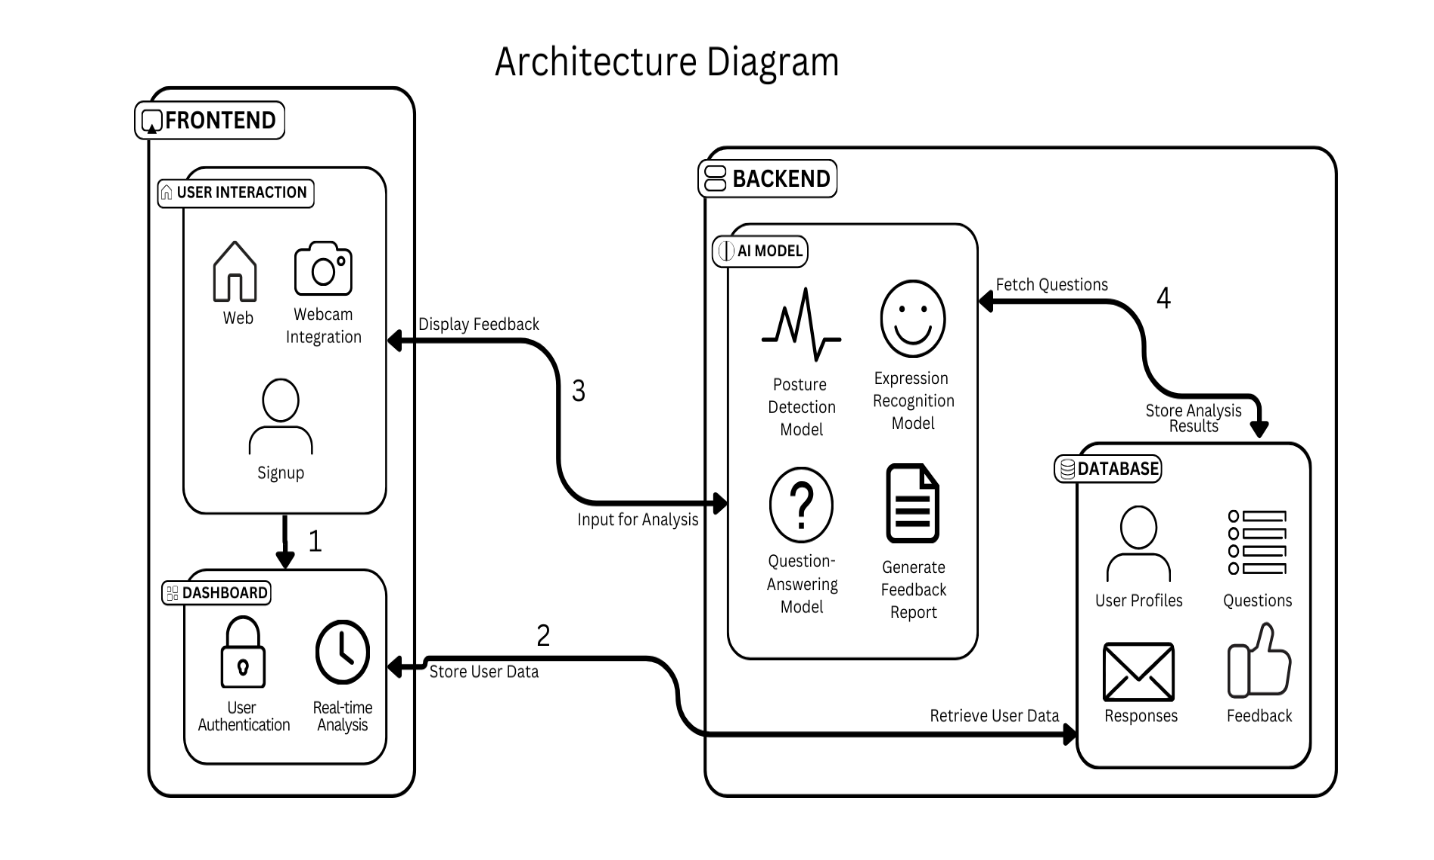
\includegraphics[width=0.8\linewidth]{sections/diagrams/ArchitectureDiagram.png}
\caption{System Architecture Diagram}
\label{fig:architecture}
\end{figure}

\begin{figure}[h]
\centering
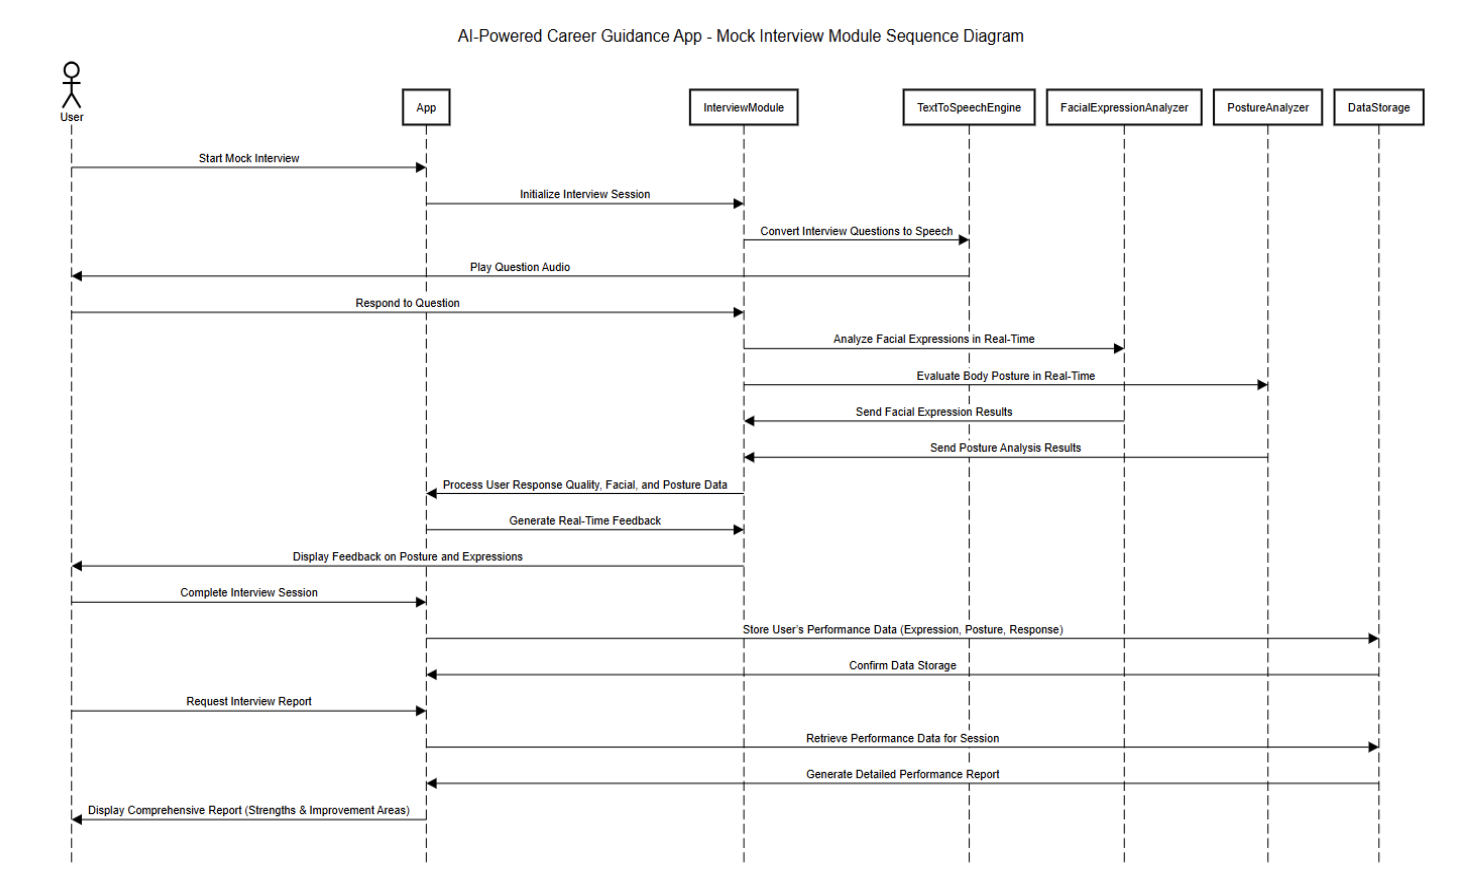
\includegraphics[width=0.8\linewidth]{sections/diagrams/SequentialModel.png}
\caption{Sequential Model Diagram}
\label{fig:sequential}
\end{figure}

\begin{figure}[h]
\centering
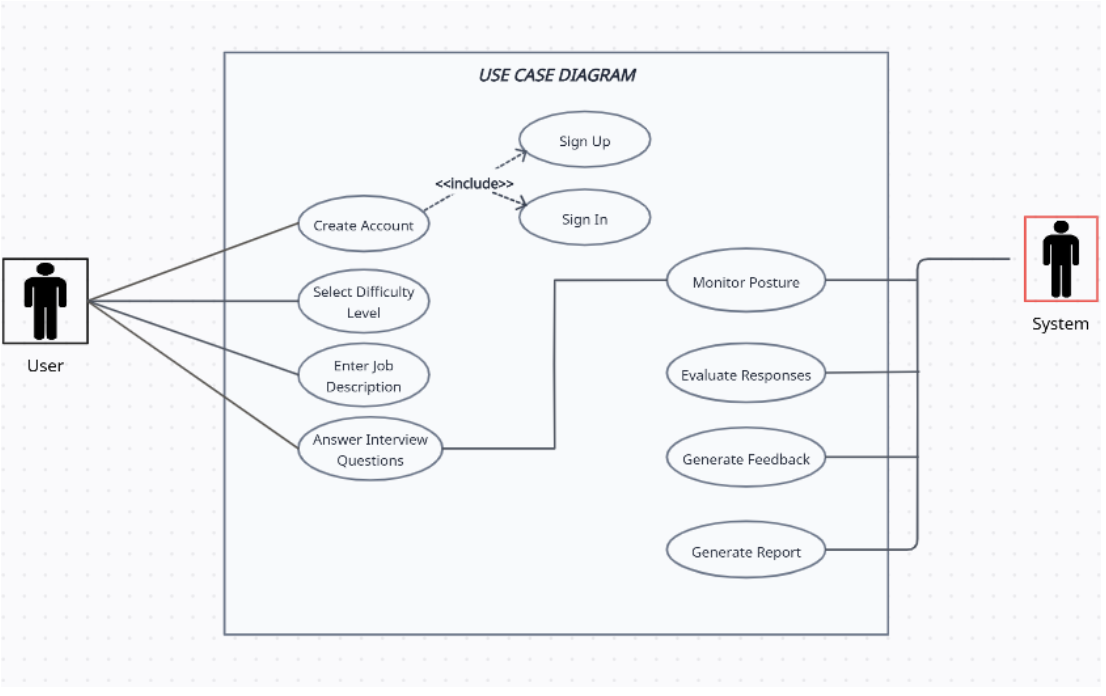
\includegraphics[width=0.8\linewidth]{sections/diagrams/UseCase.png}
\caption{Use Case Diagram}
\label{fig:usecase}
\end{figure}
